\section{Auswertung}
\label{sec:Auswertung}

%\subsection{Fehlerrechnung}
\label{sec:Fehlerrechnung}
Für die Fehlerrechnung werden folgende Formeln aus der Vorlesung verwendet.
für den Mittelwert gilt
\begin{equation}
    \overline{x}=\frac{1}{N}\sum_{i=1}^N x_i ß\; \;\text{mit der Anzahl N und den Messwerten x} 
    \label{eqn:Mittelwert}
\end{equation}
Der Fehler für den Mittelwert lässt sich gemäß
\begin{equation}
    \increment \overline{x}=\frac{1}{\sqrt{N}}\sqrt{\frac{1}{N-1}\sum_{i=1}^N(x_i-\overline{x})^2}
    \label{eqn:FehlerMittelwert}
\end{equation}
berechnen.
Wenn im weiteren Verlauf der Berechnung mit der fehlerhaften Größe gerechnet wird, kann der Fehler der folgenden Größe
mittels Gaußscher Fehlerfortpflanzung berechnet werden. Die Formel hierfür ist
\begin{equation}
    \increment f= \sqrt{\sum_{i=1}^N\left(\frac{\partial f}{\partial x_i}\right)^2\cdot(\increment x_i)^2}.
    \label{eqn:GaussMittelwert}
\end{equation}

\subsection{Bestimmung der Grenzspannung}
\label{sec:Auswertunga}

Zur Bestimmung der Grenzspannung $U_{\text{g}}$ wird eine Ausgleichsgerade durch die Messwerte gelegte. Hierbei ist zu beachten, dass die Ausgleichsgerade die linearen Abschnitte der hauptsächlich Bremsspannung umfasst.
Die Nullstelle dieser Geraden ist dann die gesuchte Spannung. Für $U_{\text{g}}$ folgt somit
\begin{equation}
    U_{\text{g}}=-a/b\, .
    \label{eqn:U_g}
\end{equation}
Die Messwerte des roten Lichtes sind in \autoref{tab:rot} tabellarisch erfasst.
\begin{table}
    \centering 
    \caption{Messwerte der roten Spektrallinie}
\begin{tabular}{c c}
    \toprule
    $U$ in V&$I$ in pA \\
    \midrule
                0.0&12 \\
                0.1&14 \\
                0.2&18 \\
                0.3&22 \\
                0.4&26 \\
                0.5&28 \\
                0.6&30 \\
                0.7&34 \\
                0.8&36 \\
                0.9&40 \\
                1.0&42 \\
                1.1&44 \\
                1.2&46 \\
                1.3&48 \\
                1.4&50 \\
                1.5&52 \\
                1.6&56 \\
                1.7&56 \\
                1.8&60 \\
                1.9&62 \\
                2.0&64 \\
                -0.1&8 \\
                -0.2&6 \\
                -0.3&4 \\
                -0.4&2 \\
                -0.5&2 \\
                -0.6&0 \\
                -0.7&0 \\
                -0.9&0 \\
                -1.1&0 \\
                -1.3&0 \\
                -1.5&0 \\
                -1.7&0 \\
                -2.0&0 \\
    \bottomrule
    \end{tabular}
    \label{tab:rot}
\end{table}
    
Die in \autoref{fig:rot} dargestellten Messwerte mit der dazugehörigen Ausgleichsgeraden liefern die Funktionsparameter 
\begin{align*}
    a_{\text{rot}}&=(4.18\pm 0.33) \, \unit{\frac{\ampere ^{1/2}}{\volt}}\\
    b_{\text{rot}}&=(3.41\pm 0.06) \, \unit{\ampere}^{1/2}\, .\\
\end{align*}
Draus folgt gemäß \autoref{eqn:U_g} ein Wert von $U_{\text{g,rot}}=(-0.82\pm 0.07)\, \unit{\volt}$.
\begin{figure}
    \centering
    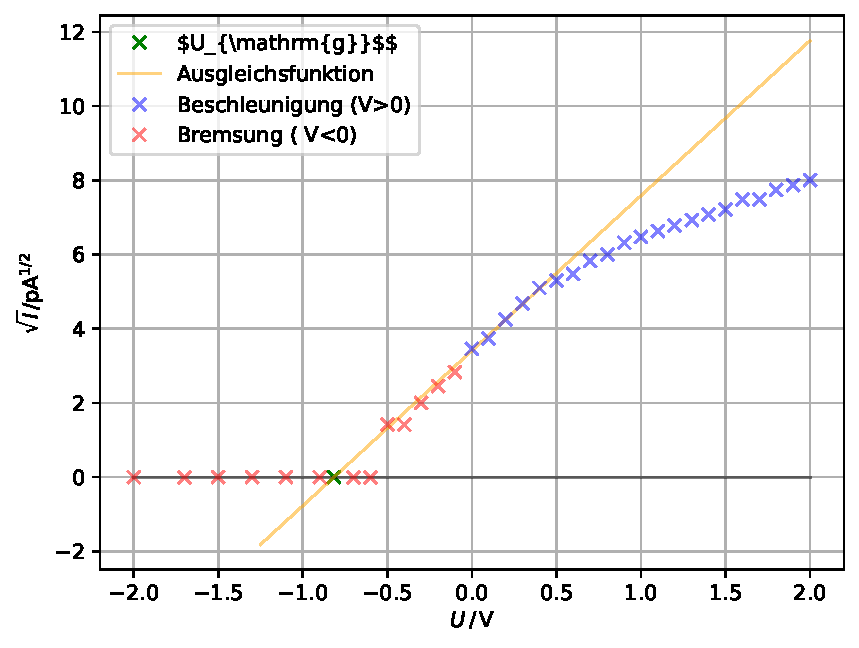
\includegraphics[height = 8cm]{build/plotrot.pdf}
    \caption{Regression zur Bestimmung der Grenzspannung $U_{\symup{g}}$ der roten Spektrallinie.}
    \label{fig:rot}
\end{figure}
Anlog zur Bestimmung von $U_{\text{g}}$ des roten Lichtes wurde die Grenzspannung der anderen beiden Wellenlängen 
berechnet.

Die Messwerte der grünen Spektrallinie sind in \autoref{tab:gruen} dargestellt.
\begin{table}
    \centering 
    \caption{Messwerte der grünen Spektrallinie}
\begin{tabular}{c c}
    \toprule
    $U$ in V&$I$ in pA \\
    \midrule
    0.00 & 500 \\
    0.10 & 580 \\
    0.20 & 620 \\
    0.30 & 700 \\
    0.40 & 760 \\
    0.50 & 840 \\
    0.55 & 880 \\
    0.60 & 900 \\
    0.65 & 940 \\
    0.70 & 940 \\
   0.80 & 1000 \\
   0.90 & 1050 \\
   1.00 & 1100 \\
   1.10 & 1150 \\
   1.20 & 1200 \\
   1.30 & 1250 \\
   1.40 & 1350 \\
   1.50 & 1400 \\
   1.60 & 1500 \\
   1.70 & 1550 \\
   1.80 & 1600 \\
   1.90 & 1700 \\
   2.00 & 1750 \\
    -0.10 & 420 \\
   -0.15 & 360 \\
    -0.20 & 320 \\
   -0.25 & 260 \\
    -0.30 & 200 \\
   -0.35 & 140 \\
    -0.40 & 100 \\
    -0.45 & 60 \\
     -0.50 & 40 \\
    -0.55 & 20 \\
      -0.60 & 0 \\
      -0.80 & 0 \\
    \bottomrule
    \end{tabular}
    \label{tab:gruen}
\end{table}

Die Messwerte und Ausgleichsgerade des grünen Lichtes ist in \autoref{fig:gruen} aufgetragen.
\begin{align*}
    a_{\text{grün}}&=(34.50\pm 1.40) \, \unit{\frac{\ampere ^{1/2}}{\volt}}\\
    b_{\text{grün}}&=(23.90\pm 0.50) \, \unit{\ampere}^{1/2}\, .\\
    \Rightarrow U_{\text{g,grün}}&=(-0.69\pm 0.03)\, \unit{\volt}\\
\end{align*}

\begin{figure}
    \centering
    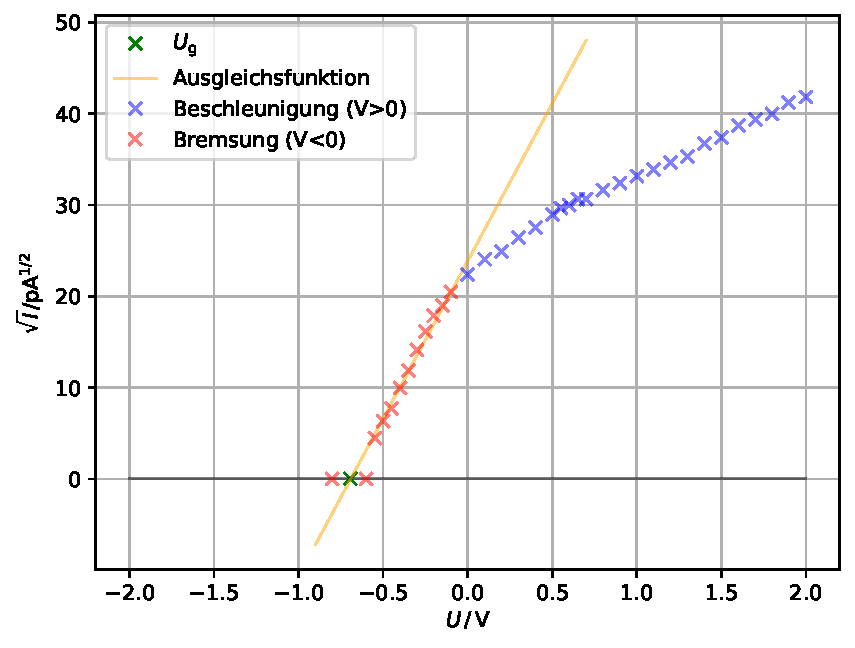
\includegraphics[height = 8cm]{build/plotgruen.pdf}
    \caption{Regression zur Bestimmung der Grenzspannung $U_{\symup{g}}$ der grünen Spektrallinie.}
    \label{fig:gruen}
\end{figure}

Die Messwerte der lila Spektrallinie sind in \autoref{tab:lila} dargestellt.
\begin{table}
    \centering 
    \caption{Messwerte der lila Spektrallinie}
\begin{tabular}{c c}
    \toprule
    $U$ in V&$I$ in pA \\
    \midrule
    0.00 & 1.00 \\
     0.10 & 1.00 \\
     0.20 & 1.20 \\
     0.30 & 1.20 \\
     0.40 & 1.40 \\
     0.50 & 1.40 \\
     0.60 & 1.60 \\
     0.70 & 1.60 \\
     0.80 & 1.60 \\
     0.90 & 1.80 \\
     1.00 & 1.80 \\
     1.10 & 1.80 \\
     1.20 & 1.90 \\
     1.30 & 1.95 \\
     1.40 & 2.15 \\
     1.50 & 2.25 \\
     1.60 & 2.35 \\
     1.70 & 2.50 \\
     1.80 & 2.55 \\
     1.90 & 2.75 \\
     2.00 & 2.95 \\
     0.00 & 0.85 \\
    -0.05 & 0.85 \\
    -0.10 & 0.80 \\
    -0.20 & 0.70 \\
    -0.30 & 0.60 \\
    -0.40 & 0.50 \\
    -0.50 & 0.40 \\
    -0.55 & 0.34 \\
    -0.60 & 0.28 \\
    -0.65 & 0.24 \\
    -0.70 & 0.18 \\
    -0.75 & 0.14 \\
    -0.80 & 0.12 \\
    -0.90 & 0.06 \\
    -1.00 & 0.02 \\
    -1.10 & 0.00 \\
    -1.20 & 0.00 \\
   -1.30 & -0.02 \\
   -1.40 & -0.02 \\
   -1.50 & -0.02 \\
   -1.60 & -0.02 \\
   -1.70 & -0.02 \\
   -1.80 & -0.02 \\
   -1.90 & -0.02 \\
   -2.00 & -0.02 \\
    \bottomrule
    \end{tabular}
    \label{tab:lila}
\end{table}
Die Messwerte und Ausgleichsgerade des violetten Lichtes ist in \autoref{fig:lila} aufgetragen.
\begin{align*}
    a_{\text{lila}}&=(0.80\pm 0.030) \, \unit{\frac{\ampere ^{1/2}}{\volt}}\\
    b_{\text{lila}}&=(0.98\pm 0.01) \, \unit{\ampere}^{1/2}\, .\\
    \Rightarrow U_{\text{g,lila}}&=(-1.22\pm 0.04)\, \unit{\volt}\\
\end{align*}

\begin{figure}
    \centering
    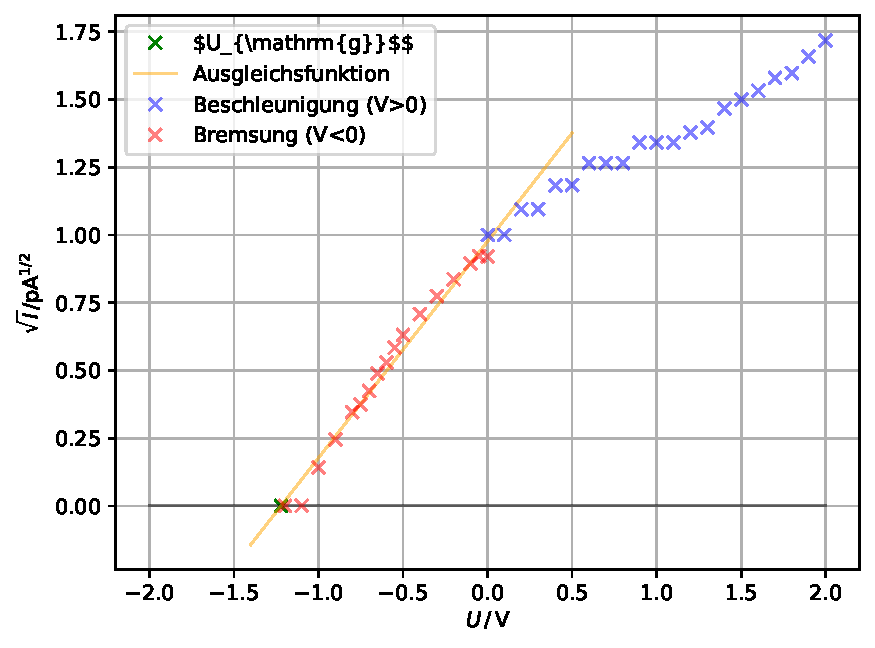
\includegraphics[height = 8cm]{build/plotlila.pdf}
    \caption{Regression zur Bestimmung der Grenzspannung $U_{\symup{g}}$ der violetten Spektrallinie.}
    \label{fig:lila}
\end{figure}

\newpage

\subsection{Bestimmung der Austrittsarbeit und des Verhältnisses $\frac{h}{e_0}$}
\label{sec:Auswertungb}

In \autoref{tab:freq} befinden sich die Wellenlängen, die Frequenz und die zugehörige Grenzspannung. 
\begin{table}
    \centering 
    \caption{Wellenlänge, Frequenz und zugehörige Grenzspannung.}
\begin{tabular}{c c c}
    \toprule
    $\lambda$ in nm &$\nu$ in $10^{14}\cdot$\,Hz & $U_{\symup{g}}$ in V  \\
    \midrule
    700 & 4.28271 & 0.8158\\ 
546 & 5.49066 & 0.6930\\
435 & 6.89172 & 1.2215\\
    \bottomrule
\end{tabular}
\label{tab:freq}
\end{table}

Die Frequenz wurde dabei mit
\begin{equation*}
    \nu = \frac{\symup{c}}{\lambda}
\end{equation*}
berechnet. Die Wellenlängen wurden vorwiegend der Versuchsanleitung \cite{ap500} entnommen. Für die Wellenlänge von rotem Licht wurde 
$700\,\unit{\nm}$ \cite{rot} gewählt.
In \autoref{fig:freq} wurde nun der jeweilige Betrag Grenzspannung gegen die Frequenz aufgetragen und eine Ausgleichsrechnung mittels einer Geraden 
\begin{equation*}
    y = ax+b
\end{equation*}
durchgeführt.
\begin{figure}
    \centering
    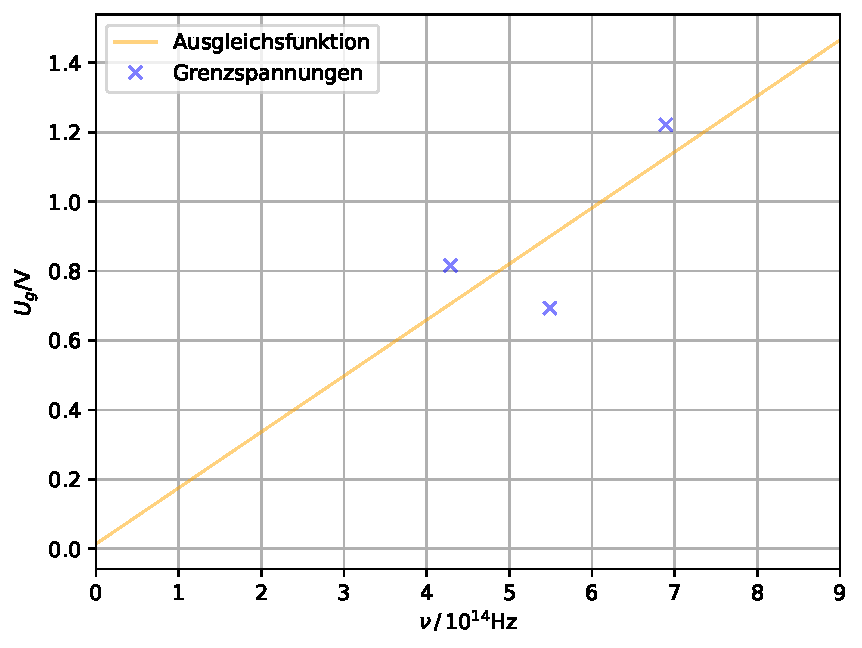
\includegraphics[height = 8cm]{build/frequenz.pdf}
    \caption{Verlauf der Grenzspannungen in Abhängigkeit von der Frequenz.}
    \label{fig:freq}
\end{figure}
Dabei ergeben sich für die Steigung, welche hier nach \autoref{eqn:nu} das Verhältnis $\frac{h}{\symup{e_0}}$ darstellt 
\begin{equation*}
    a = \frac{h}{\symup{e_0}} = (1.614 \pm 1.372) \cdot 10^{-15} \,\symup{Vs}
\end{equation*}
und den y-Achsenabschnitt
\begin{equation*}
    b = A_{\symup{k}} = (0.014 \pm 0.776) \,\unit{\eV} \; ,
\end{equation*}
welcher hier der Austrittsarbeit $A_{\symup{k}}$ entspricht.




In \autoref{fig:gelb} wird der Verlauf des Photostroms bei einer Wellenlänge von $\lambda = 578 \,\unit{\nm}$ dargestellt. Dabei wurde ein größeres 
Intervall der anliegenden Spannung betrachtet. Die dazu gehörenden Messwerte finden sich in \autoref{tab:gelb}.

\begin{table}
    \centering 
    \caption{Messwerte der gelben Spektrallinie.}
\begin{tabular}{c c}
    \toprule
    $U$ in V&$I$ in pA \\
    \midrule
    0&60 \\
    1&180 \\
    2&280 \\
  2.5&320 \\
    3&380 \\
  3.5&400 \\
    4&440 \\
  4.5&440 \\
    5&460 \\
    6&500 \\
    7&520 \\
    8&540 \\
    9&560 \\
   10&580 \\
   11&580 \\
   12&640 \\
   13&640 \\
   14&660 \\
   15&660 \\
   16&680 \\
   17&700 \\
   18&700 \\
   19&720 \\
    0&180 \\
    -1&20 \\
    -3&20 \\
    -4&15 \\
    -5&15 \\
    -6&15 \\
    -7&15 \\
    -8&15 \\
    -9&18 \\
   -10&18 \\
   -11&18 \\
   -12&20 \\
   -13&20 \\
   -14&20 \\
   -15&20 \\
   -16&20 \\
   -17&20 \\
   -18&20 \\
   -19&20 \\
    \bottomrule
\end{tabular}
\label{tab:gelb}
\end{table}

    
\begin{figure}
    \centering
    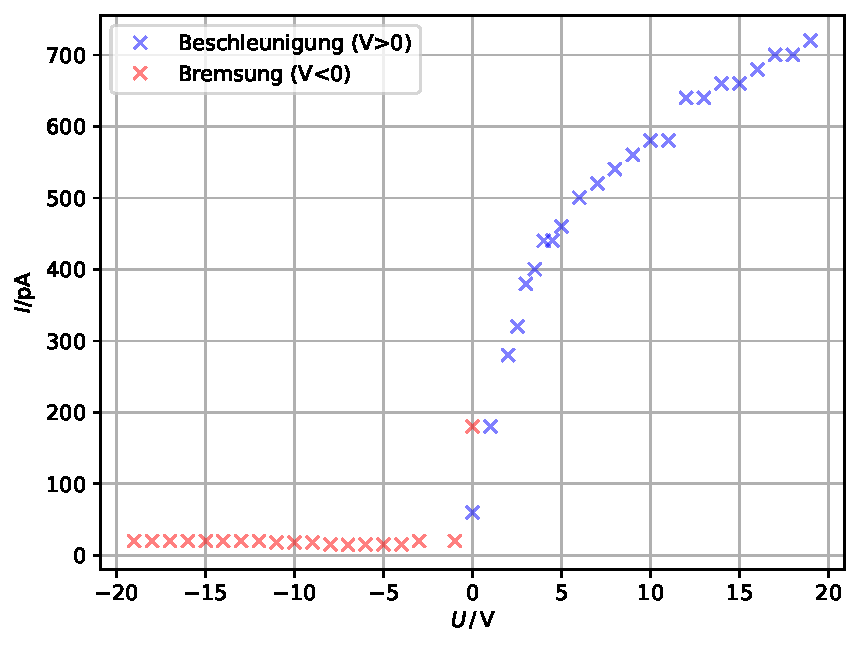
\includegraphics[height = 8cm]{build/plotgelb.pdf}
    \caption{Verlauf des Photostroms der gelben Spektrallinie bei $\lambda = 578 \,\unit{\nm}$.}
    \label{fig:gelb}
\end{figure}
Bei hohen beschleunigenden Spannung erreicht der Photostrom asymptotisch einen Sättigungswert. Dies liegt daran, dass ab einer bestimmten
Beschleunigungsspannung alle Elektronen die Anode erreichen. Nach der Korpuskeltheorie ist die Anzahl der Elektronen proportional zur Intensität 
des Lichts, sodass bei konstanter Lichteinstrahlung der obigen Wellenlänge der Strom nicht über einen bestimmten Wert hinauswachsen kann. In 
\autoref{fig:gelb} erkennt man bei großen Beschleunigungsspannungen langsam eine Abflachung des Strom; der Sättigungswert ist jedoch noch nicht ganz erkennbar.
Die Annäherung an dem Sättigungswert erfolgt asymptotisch und der Sättigungswert kann in der Praxis nicht vollständig erreicht werden. Dies liegt daran ,dass 
nicht alle Elektronen durch etwaige Ablenkungen und Widerstände die Anode erreichen können. Bei hohen Beschleunigungen haben diese aber einen immer geringeren 
Einfluss. Um den Sättigungswert zu erreichen müssen also alle Widerstände und Ablenkungen eliminiert werden. Das ist nur im Vakuum und bei einer ausreichenden 
Isolierung und Abschirmung von anderen Lichtquellen der  gesamten Messapparatur möglich.

Der Photostrom fällt bei $U_{\symup{g}}$ nicht direkt auf Null ab, da die Elektronen schon vor der Emission aus dem Material eine gewisse Energie 
haben, welche der Fermi-Dirac-Statistik folgt. Dadurch werden größere Bremsspannungen benötigt, um alle Elektronen soweit auszubremsen, dass sie die 
Anode nicht erreichen. In \autoref{fig:gelb} wird die Null gar nicht erreicht, da die Bremsspannungen scheinbar noch nicht groß genug sind. Dennoch erkennt 
man direkt unter einer Spannung von $0\,\unit{\volt}$ einen etwas höheren Photostrom als bei größeren Bremsspannungen, was darauf hindeutet, dass 
der Photostrom noch weiter abfallen wird, wenn die Bremsspannung weiter erhöht werden würde.

Grundsätzlich kann ein kleiner entgegengerichteter Strom bei hohen Bremsspannungen gemessen werden. Bei dem Versuchsteil zur gelben Spektrallinie wurde dies jedoch nicht beobachtet 
Bei der violetten Spektrallinie in \autoref{tab:lila} jedoch schon. Dieser ist damit zu erklären, dass das Kathodenmaterial bei $T=20°\,\unit{\celsius}$ 
verdampft, wodurch Elektronen freigesetzt werden und sich an der Anode anlagern. Das führt dazu, dass die Elektronen wegen der hohen Bremsspannung von der 
Anode wegbeschleunigt werden und es wird ein negativer Strom gemessen. Dadurch dass hierbei wesentlich weniger Elektronen zu beobachten sind, kann hier 
der Sättigungswert erreicht werden. 

Da der negative Strom bereits bei energiearmen Licht beobachtet werden kann, muss die Austrittsarbeit mindestens so klein wie die der Kathode sein.

